\chapter{Defect chemistry and \ce{Li} ion diffusion in \ce{Li4Mn2O5}}
\section{Background}
Defect chemistry and the pathways that govern ion diffusion in electrodes are of vital importance to understanding the electrochemical performance of potential battery materials.
These parameters can not be determined by experimental methods alone, requiring atomistic or DFT studies to study migration barriers and understand the direction and dimensionality of lithium ion motion.

As discussed in Chapter 1, there has been recent interest in disordered rock-salts as next-generation cathode materials.
\ce{Li4Mn2O5}, one such material, offers capacities (\SI{355}{\milli\ampere\hour\per\gram}) which far exceed those seen in conventional cathodes, and uses non-toxic and earth-abundant manganese in place of cobalt.
The aim of this section is to investigate the intrinsic defect chemistry and lithium diffusion properties of \ce{Li4Mn2O5}, which are yet to be studied in depth or properly understood.
Further, the highly disordered nature of this material presents challenges to the use of certain computational methods, so a range of atomistic modelling techniques are applied to identify those suited to this and similar issues.

\newpage
\begin{figure}[h]
\centering
\vspace{1cm}
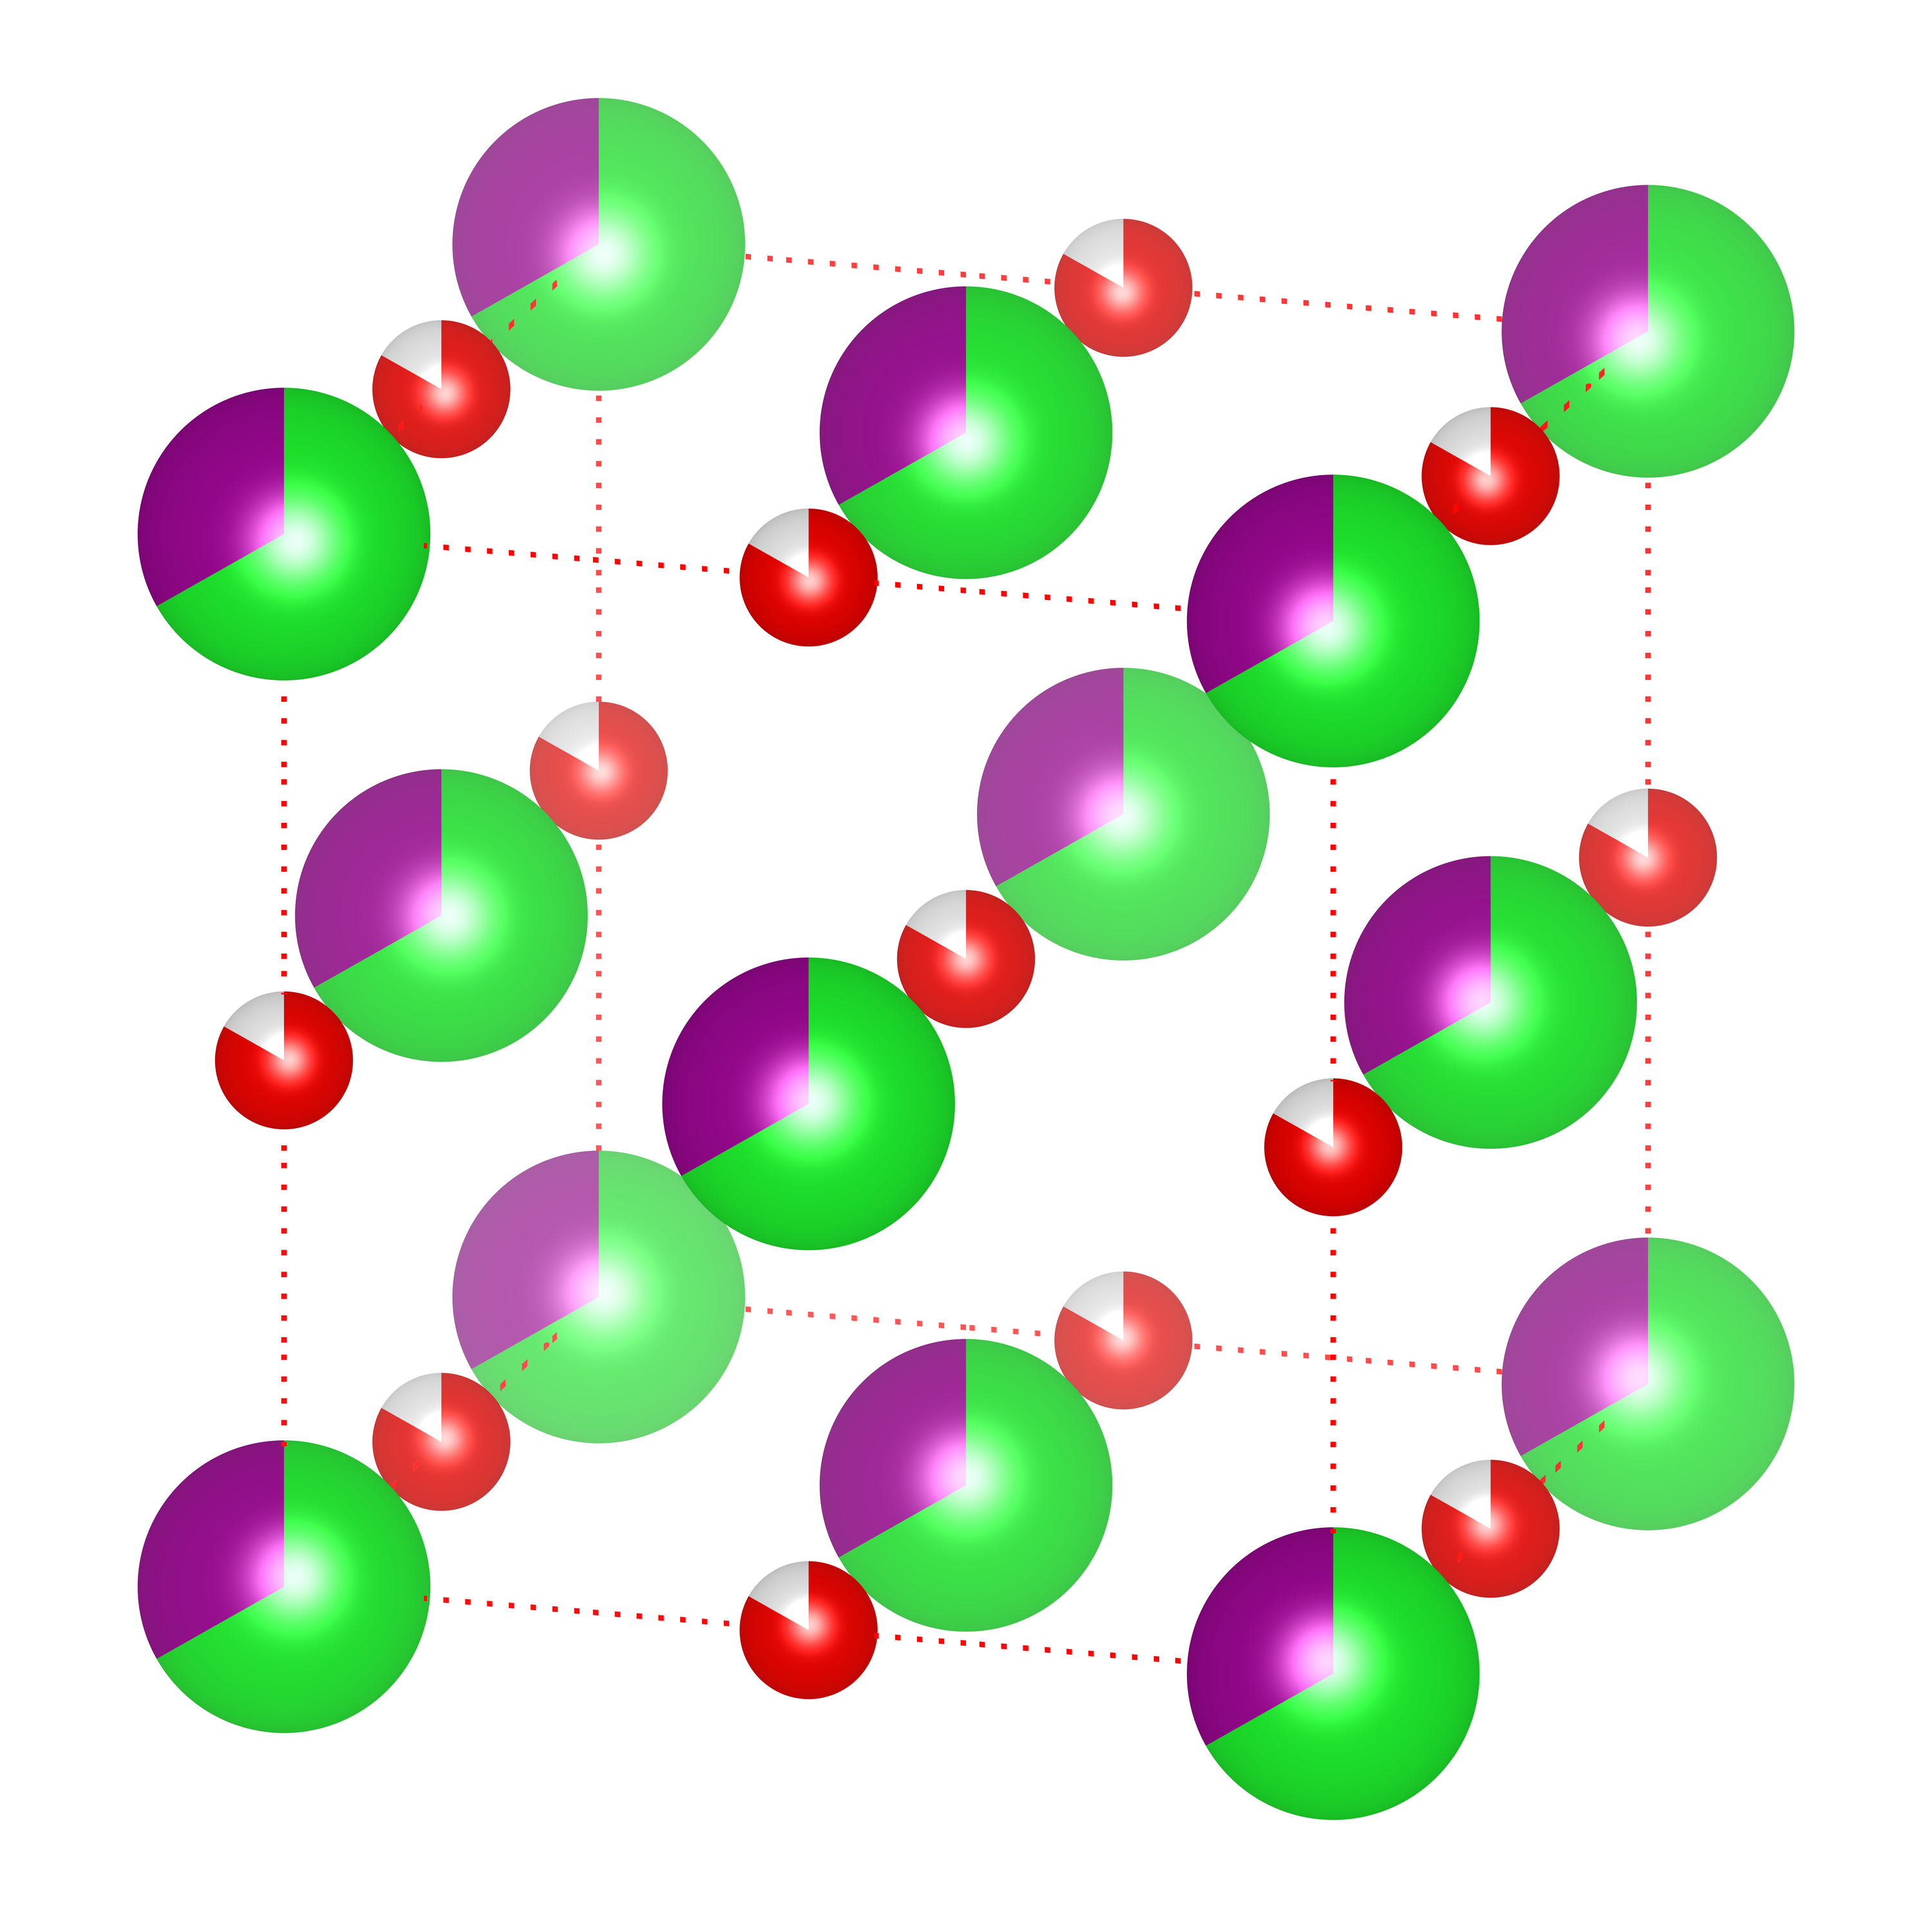
\includegraphics[width=0.8\linewidth]{figures/structures/Li4Mn2O5_compressed}
\caption[Crystal structure of \ce{Li4Mn2O5}]{Crystal structure of \ce{Li4Mn2O5}, showing an average \ce{MnO} rock-salt structure (space-group 225) with the random substitution of 2/\nth{3}\textsuperscript{s} of \ce{Mn} sites with Li, charge compensated by 1/\nth{6} of oxygen sites being vacant.. Li ions: green; Mn ions: purple; \ce{O} ions: red. Each lattice site shows a pie chart, corresponding to the occupancy of that site.}
\label{fig:Li4Mn2O5-average}
\end{figure}

\section{Structure generation and modelling}
While no ordering is noted in experimental work,\cite{Freire2016,Diaz-Lopez2018a} computational studies have identified a number of ordered structures which lower energies than pseudo-random structures generated for comparison.\cite{Diaz-Lopez2017,Bhandari2019}

\newpage
\subsection{Mean-field approximation}
The mean-field approximation can be used to study systems with partially occupied sites without the need to assign either a vacancy or given species to each site.
This is a useful exercise for the purposes of validating potential parameters against experimental lattice parameters.
The potential parameters used to study this system were taken from past work in the literature on lithium manganese oxides by \citet{Ammundsen1999}, and are listed in Table \ref{tab:potentials}, although i

The calculated lattice parameters give good agreement with the experimental structure (within $2.5\%$).
It is noted in the literature that local deviations from the rock-salt structure arising from structural disorder give rise to a broad range of inter-atomic spacings.\cite{Yahia2019}

\begin{table}[h]
\centering
\caption[Two-body short-range potential parameters for \ce{Li4Mn2O5}]{Two-body short-range potential parameters for \ce{Li4Mn2O5}.\cite{Ammundsen1999}}
\begin{tabular}{@{}lS[table-format=5.2]S[table-format=1.4]S[table-format=2.1]S[table-format=1.2]S[table-format=5.1]@{}}
\toprule
\textbf{Interaction} &\multicolumn{1}{c}{\textbf{A} (\si{\electronvolt})}   & \multicolumn{1}{c}{$\boldsymbol{\rho}$ (\AA)} & \multicolumn{1}{c}{\textbf{C} (\si{\electronvolt \angstrom \tothe{6}})} & \multicolumn{1}{c}{\textbf{Y} (e)}& \multicolumn{1}{c}{\textbf{K} (\si{\electronvolt \angstrom \tothe{-2}})}\\
\midrule
\ce{Li+ -\;O^2-}   & 426.48  & 0.300                          & 0.0  & 1.0        & 99999.0 \\
\ce{Mn^3+ -\;O^2-}       & 1267.5  & 0.3240                         & 0.0  & 3.00       & 850.0   \\
\ce{O^2- -\;O^2-}        & 22764.3 & 0.1490                         & 43.0 & -2.96      & 57.0\\
\bottomrule
\end{tabular}
\label{tab:potentials}
\end{table}


\newcommand{\tableline}{\multicolumn{1}{c}{--}}
\newcommand{\tableliner}{\multicolumn{1}{c}{{\color{red}--}}}
\newcommand{\mc}[1]{\multicolumn{1}{c}{#1}}

\begin{table}[h]
\centering
\caption{Calculated lattice parameters of \ce{Li4Mn2O5} using mean-field approximation compared to experimental data.}
\begin{tabular}{lS[table-format=1.4]S[table-format=2.1]}
\toprule
\textbf{Lattice parameter} &\mc{\textbf{a} = \textbf{b} = \textbf{c} (\AA)} & \mc{$\boldsymbol{\alpha} = \boldsymbol{\beta} = \boldsymbol{\gamma}$ (\si{\degree})}\\
\midrule
Experimental \cite{Freire2016} &  4.1733  & 90.0 \\
Mean-field                     &  4.0705  & 90.0 \\ 
\textit{$\Delta$}              & -0.1028  & 0.0  \\
\textit{$\Delta$ (\%)}         & -2.46    & 0.0  \\\bottomrule
\end{tabular}
\end{table}
\newpage

\subsection{Disordered structure generation}
In the absence of prior information regarding the stability of given local environments, structures were randomly generated.
Twenty such structures were produced, ten containing 216 atoms and the other ten containing 1728 atoms, with each site randomly assigned an atom in accordance with the occupancy of that site.
These supercell sizes were chosen to give stoichiometrically correct systems with an integer number of species.
A number of these structures contained local environments not numerically stable with the potential parameters used, leading to these simulations crashing.

Table \ref{tab:randomresults} gives the lattice parameters of each of the relaxed random structures which converged, with cell lengths scaled for direct comparison with experimental data.\cite{Freire2016}
Some structures give good agreement with experimental lattice parameters (e.g. 1728 atoms, model 9), however some other randomly generated structures have cell lengths which differ from experiment by over 7 percent.%, suggesting that random structure generation does not produce structures which reliably agree with experiment.
Even for those structures which do closely match experimental lattice parameters, local deviations of atom positions are huge, suggesting that either the potential parameters selected are not suitable for the material or that randomly generating structures in this manner leads to unphysical local environments forming. This can be seen in Figure \ref{fig:random}, which is representative of the distortions seen in all randomly generated structures upon relaxation.

\newpage
\begin{landscape}
\begin{table}[h]
\centering
\caption{Calculated lattice parameters of \ce{Li4Mn2O5} for randomly generated structures compared to experimental data, including only those configurations (\#) which did not converge.}
\begin{tabular}{lr @{\hskip 1cm} *{3}{d{1.4}} *{3}{d{3.1}} @{\hskip 1cm} *{6}{d{2.2}}}
\toprule
&&\multicolumn{6}{c}{Lattice parameter}&\multicolumn{6}{c}{$\Delta$ (\%)}\\
\cmidrule(lr){3-8}
\cmidrule(lr){9-14}
\textbf{Case} &\textbf{\#}&\mc{\textbf{a} (\AA)}   & \mc{\textbf{b} (\AA)} & \mc{\textbf{c} (\AA)}& \mc{$\boldsymbol{\alpha}$ (\si{\degree})} & \mc{$\boldsymbol{\beta}$ (\si{\degree})} & \mc{$\boldsymbol{\gamma}$ (\si{\degree})} &\mc{\textbf{a}}   & \mc{\textbf{b}} & \mc{\textbf{c}}& \mc{$\boldsymbol{\alpha}$} & \mc{$\boldsymbol{\beta}$} & \mc{$\boldsymbol{\gamma}$}\\
\midrule \vspace{0.5cm}
Experimental \cite{Freire2016}& & 4.1733  & 4.1733 & 4.1733 & 90.0 & 90.0 & 90.0 &\tableline &\tableline &\tableline &\tableline &\tableline &\tableline \\ 
216 atoms & 1 & 3.9236 & 4.3417 & 4.2291 & 89.1 & 89.1 & 88.8 & 5.98 & -4.04 & -1.34 & 0.95 & 1.00 & 1.35\\ 
& 8 & 4.2818 & 3.9504 & 4.3069 & 88.2 & 90.0 & 90.1 & -2.60 & 5.34 & -3.20 & 2.05 & 0.01 & -0.07\\ 
& 9 & 4.0880 & 4.0162 & 4.4424 & 88.5 & 89.6 & 89.2 & 2.04 & 3.76 & -6.45 & 1.69 & 0.44 & 0.87\\ \vspace{0.5cm}
& 10 & 4.0871 & 4.5213 & 3.9217 & 91.1 & 87.9 & 87.6 & 2.07 & -8.34 & 6.03 & -1.19 & 2.37 & 2.66\\ 
1728 atoms & 1 & 3.8624 & 4.4443 & 4.1821 & 88.7 & 90.1 & 89.6 & 7.45 & -6.50 & -0.21 & 1.42 & -0.06 & 0.50\\ 
& 2 & 3.9664 & 4.3081 & 4.2099 & 90.9 & 90.7 & 88.8 & 4.96 & -3.23 & -0.88 & -1.05 & -0.75 & 1.31\\ 
& 4 & 4.1231 & 4.1710 & 4.1417 & 90.1 & 90.1 & 89.4 & 1.20 & 0.06 & 0.76 & -0.06 & -0.06 & 0.67\\ 
& 5 & 4.0915 & 4.2965 & 4.1210 & 89.5 & 89.5 & 89.9 & 1.96 & -2.95 & 1.25 & 0.57 & 0.53 & 0.06\\ 
& 7 & 4.0180 & 4.3784 & 4.0803 & 90.3 & 90.2 & 89.5 & 3.72 & -4.92 & 2.23 & -0.36 & -0.23 & 0.59\\ 
& 8 & 4.1189 & 4.3067 & 4.0170 & 90.6 & 89.1 & 88.6 & 1.30 & -3.20 & 3.74 & -0.69 & 1.03 & 1.52\\ 
& 9 & 4.1648 & 4.1826 & 4.1599 & 90.1 & 91.0 & 89.8 & 0.20 & -0.22 & 0.32 & -0.15 & -1.14 & 0.22\\ 
& 10 & 4.0773 & 4.3573 & 4.1014 & 90.9 & 90.2 & 89.6 & 2.30 & -4.41 & 1.72 & -1.00 & -0.22 & 0.49\\ \bottomrule
\end{tabular}
\label{tab:randomresults}
\end{table}
\end{landscape}
\newpage
\begin{figure}[H]
\centering
 \begin{subfigure}{\textwidth}
 \centering
    \includegraphics[height=0.4\textheight]{figures/structures/random_initial}
    \caption{Initial structure}
    \label{fig:random_initial}
 \end{subfigure}
  \begin{subfigure}{\textwidth}
   \centering
    \includegraphics[height=0.4\textheight]{figures/structures/random_final}
    \caption{Relaxed structure}
    \label{fig:random_final}
 \end{subfigure}
\caption{Comparison of the initial and final structures obtained by relaxing a randomly generated 1728 atom (configuration 9) \ce{Li4Mn2O5} disordered rock-salt.}
\label{fig:random}
\end{figure}

\newpage
\subsection{Ordered structures}
\label{sec:ordered}
As the generation of random structures led to unstable simulations for MD studies, irrespective of the potential parameters selected, ordered structures were taken from literature as a basis for structural modelling.
\citet{Diaz-Lopez2017} used Enum, a structure enumeration tool, to search for the lowest energy ordered \ce{Li4Mn2O5} structure up to a 24 atom system, using DFT to relax and determine the lattice energy of each system.
The resultant ground-state structure, shown in Figure \ref{fig:random_initial}, is used in this work.
The calculated lattice parameters give good agreement with literature, within 2.5\% of the relaxed DFT structure from the literature.
Additionally, as can be seen in Figure \ref{fig:random}, there is minimal movement of atoms from their initial sites.
This agreement with DFT data serves to validate the suitability of the interatomic potentials used for modelling this system.
\vfill
\begin{table}[h]
\centering
\caption{Calculated lattice parameters of ordered \ce{Li4Mn2O5} compared to DFT data.}
\begin{tabular}{lS[table-format=4.4]S[table-format=4.4]S[table-format=4.4]S[table-format=2.1]}
\toprule
\textbf{Lattice parameter} &\mc{\textbf{a} (\AA)}   & \mc{\textbf{b} (\AA)} & \mc{\textbf{c} (\AA)}&\mc{$\boldsymbol{\alpha} = \boldsymbol{\beta} = \boldsymbol{\gamma}$ (\si{\degree})}\\
\midrule
DFT structure \cite{Diaz-Lopez2017} &  4.0390  & 12.4312 &  4.0268 & 90.0 \\
This work                           &  3.9446  & 12.3911 &  3.9541 & 90.0 \\ 
\textit{$\Delta$}                   & -0.0944  & -0.0401 & -0.0726 &  0.0 \\
\textit{$\Delta$ (\%)}              & -2.34    & -0.32   & -1.80   &  0.0 \\ \bottomrule
\end{tabular}
\end{table}
\vspace{0.25\textheight}

\begin{figure}[p]
\centering

\begin{subfigure}{0.5\textwidth}
\centering
\includegraphics[width = 0.9\linewidth]{figures/structures/ordered_in}
\caption{Input structure\cite{Diaz-Lopez2017}}
\end{subfigure}%
\begin{subfigure}{0.5\textwidth}
\centering
\includegraphics[width = 0.9\linewidth]{figures/structures/ordered_in}
\caption{Relaxed structure}
\end{subfigure}

\caption[Comparison of the initial and relaxed structures for ordered \ce{Li4Mn2O5}]{Comparison of the initial and relaxed structures for \ce{Li4Mn2O5}, with ordering as proposed by \citet{Diaz-Lopez2017}.}
\end{figure}

\newpage
\begin{figure}[h] %TODO Try alternate labelling scheme for sites
\centering
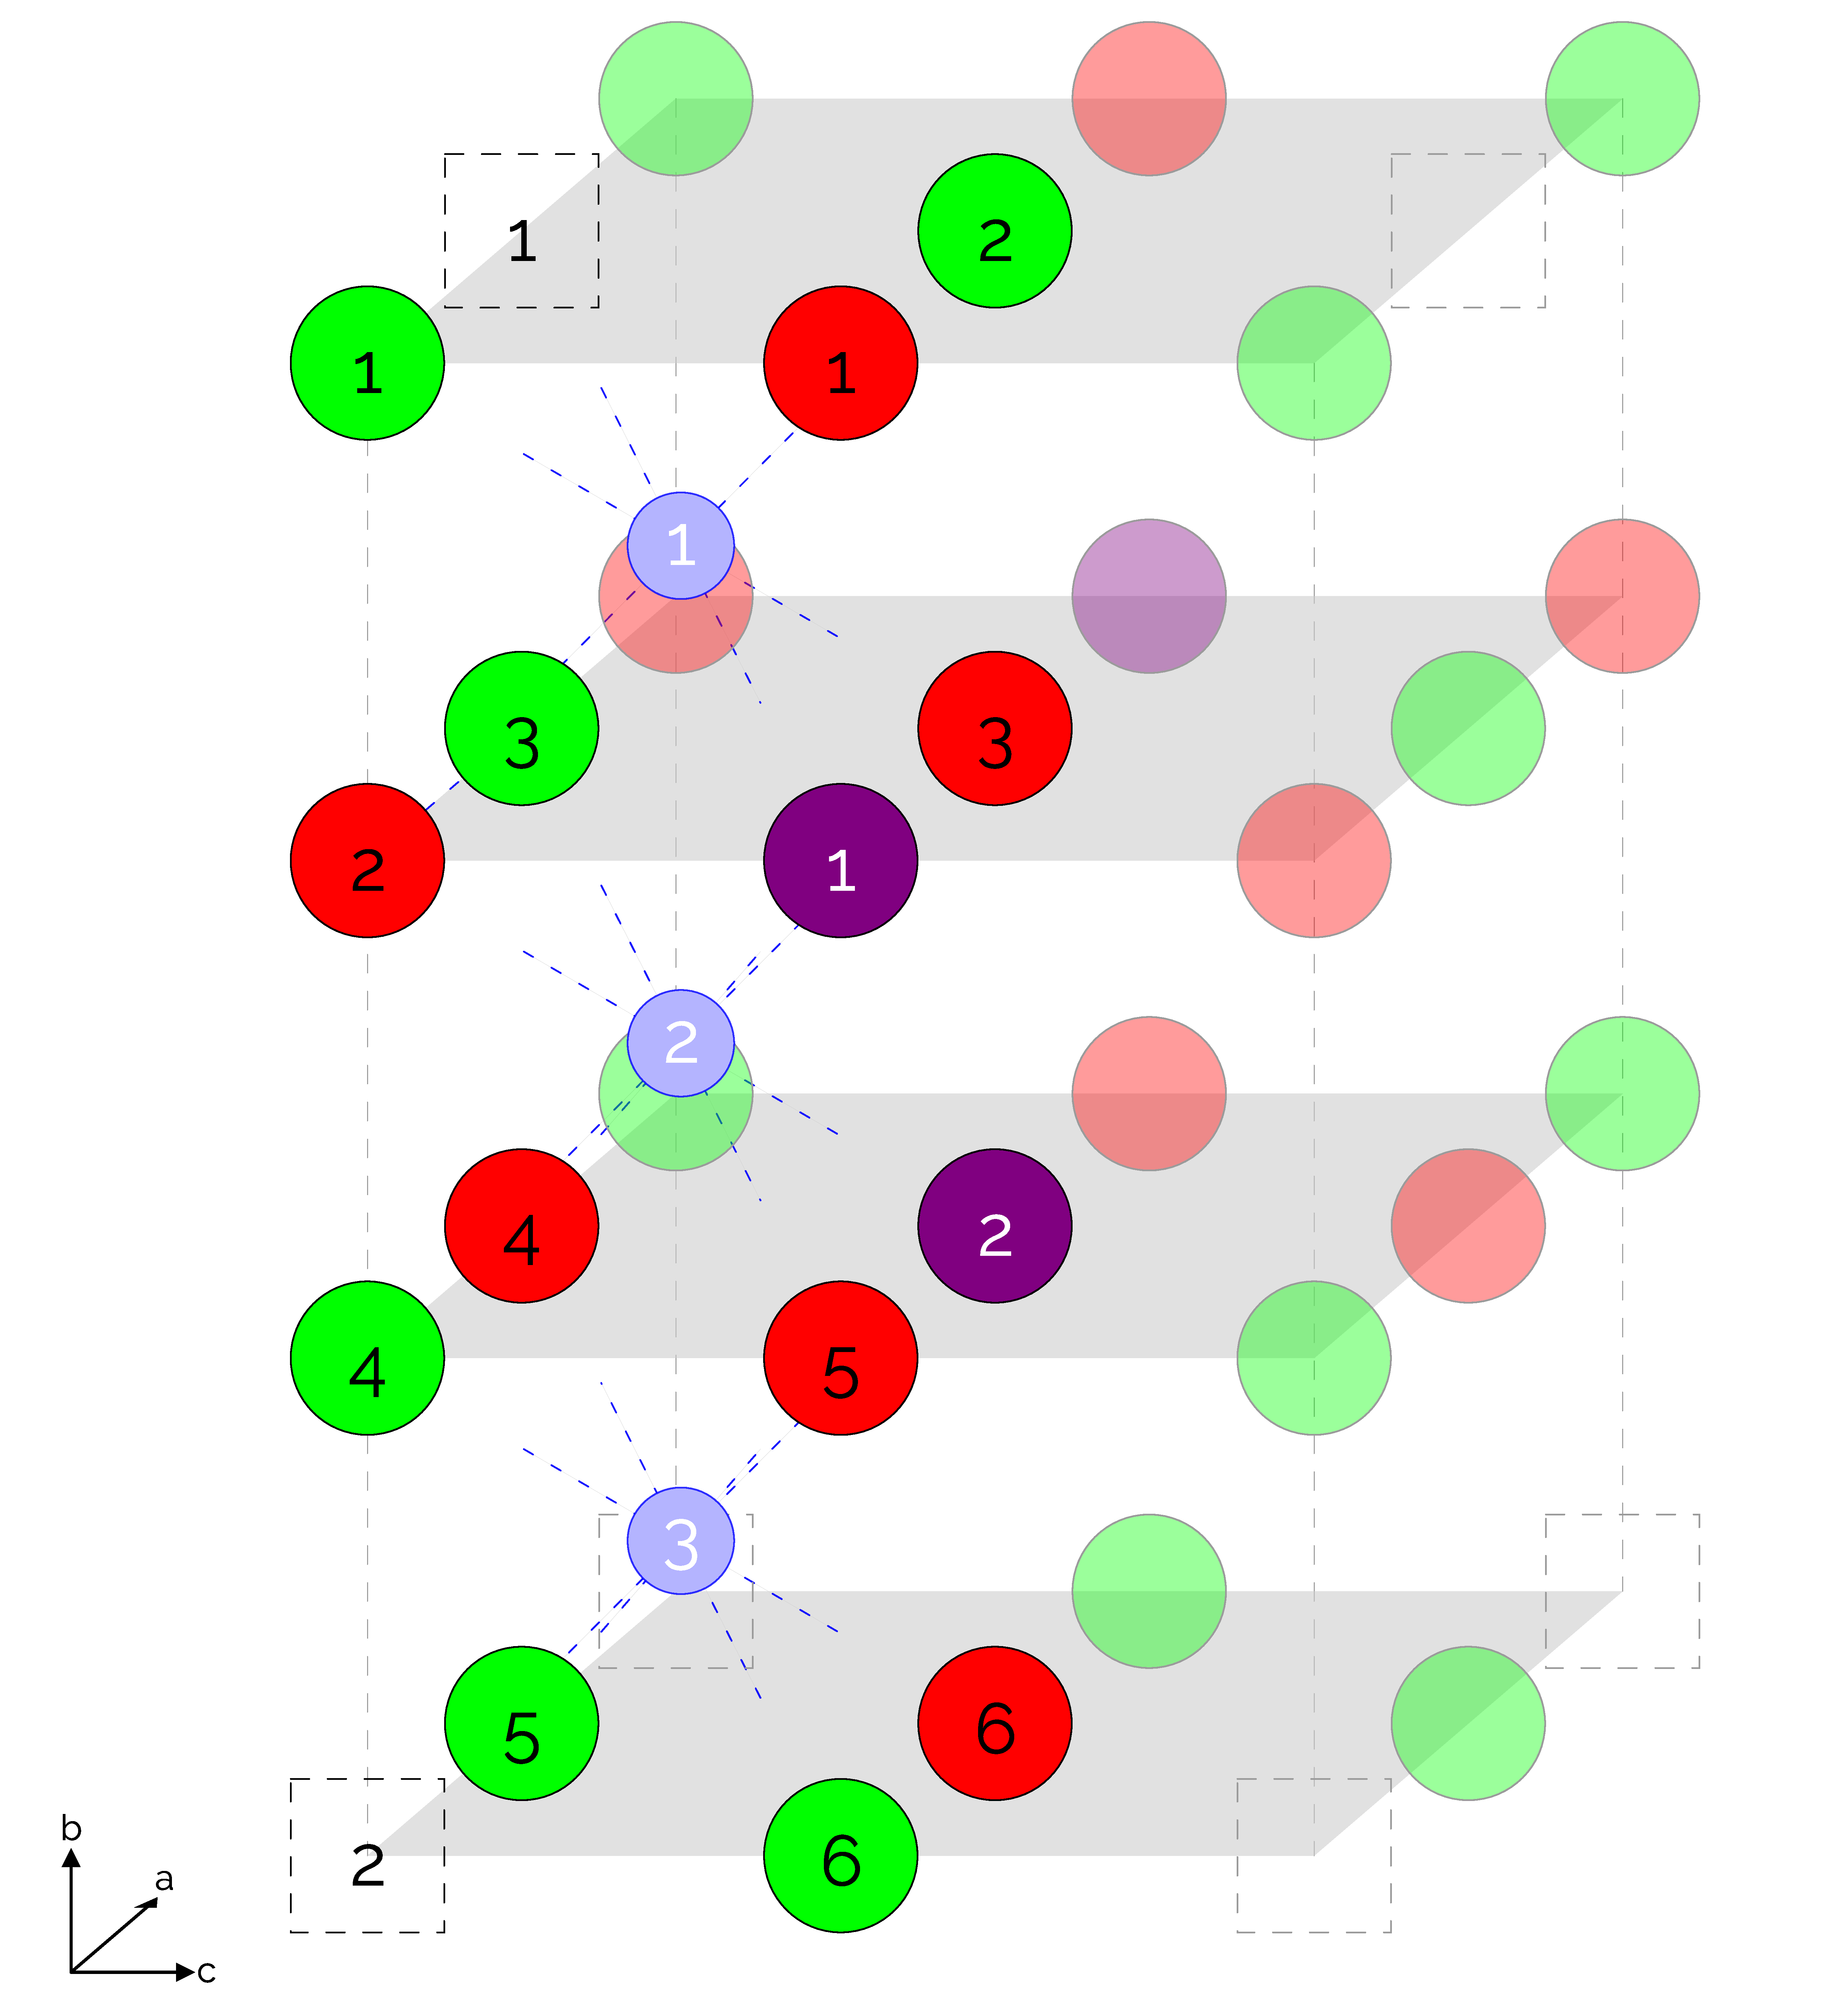
\includegraphics[height = 0.55\textheight]{figures/orderedlabels/orderedlabels}
\caption[Site labelling scheme for ordered \ce{Li4Mn2O5}]{Site labelling scheme for ordered \ce{Li4Mn2O5}. A reflection at either the top or bottom plane yields the structure previously proposed.\cite{Diaz-Lopez2017} Li ions: green; Mn ions: purple; O atoms: red; O vacancies: dashed squares; Interstitial sites: blue.
}
\label{fig:orderedlabel}
\end{figure}

\section{Intrinsic atomic defects}
Using the ordered structure from Section \ref{sec:ordered}, a series of point defect calculations were calculated, allowing for the formation energies of Schottky, Frenkel, and anti-site defects to be determined.
Figure \ref{fig:orderedlabel} shows the labelling scheme used to refer to each symmetrically unique site in the structure throughout this section.
\newpage
\begin{table}[p]
\centering
\caption{Isolated defect formation energies in ordered \ce{Li4Mn2O5}.}
\vspace{0.5cm}
\begin{subtable}{\linewidth}\centering
\caption{Vacancies.}
\begin{tabular}{l *{3}{d{2.2}}}
\toprule
&\multicolumn{3}{c}{Energy (eV)}\\
\cmidrule(lr){2-4}
\textbf{Site (n)} & \mc{$\ce{V_{Li}}$} & \mc{$\ce{V_{Mn}}$} & \mc{$\ce{V_{O}}$}\\
\midrule
1 & 6.93 & 46.19 & 24.77 \\
2 & 5.57 & 46.19 & 23.24 \\
3 & 7.26 & \tableline & 24.61 \\
4 & 7.26 & \tableline & 23.24 \\
5 & 6.93 & \tableline & 24.61 \\
6 & 5.57 & \tableline & 24.77 \\
\midrule
Minimum & 5.57 & 46.19 & 23.24  \\
\bottomrule
\end{tabular}
\label{tab:vacancies}
\end{subtable}
\vspace{1cm}

\begin{subtable}{\linewidth}\centering
\caption{Interstitial defects; 1 -- 3 refer to interstices, whilst V1 and V2 refer to vacant O sites.}
\begin{tabular}{l *{3}{d{3.2}}}
\toprule
&\multicolumn{3}{c}{Energy (eV)}\\
\cmidrule(lr){2-4}
\textbf{Site (n)} & \mc{$\ce{Li_{i}}$} & \mc{$\ce{Mn_{i}}$} & \mc{$\ce{O_{i}}$}\\
\midrule
1 & -3.85 & -36.41 & \tableline \\
2 & -3.80 & -36.71 & -17.09 \\
3 & -3.85 & -36.41 & \tableline \\
V1 & -2.94 & -36.12 & -20.16 \\
V2 & -2.94 & -36.12 & -20.16 \\
\midrule
Minimum & -3.85 & -36.71 & -20.16  \\
\bottomrule
\end{tabular}
\label{tab:interstitial}
\end{subtable}
\label{tab:primitivedefects}
\end{table}

\clearpage
\noindent
Table \ref{tab:primitivedefects} shows the isolated energies of vacancies and interstitial defects at each site labelled in Figure \ref{fig:orderedlabel}.
Oxygen interstitial defects introduced at interstices 1 and 3 displace into the adjacent oxygen vacancy, with only interstitial site 2 able to host stable interstitial oxygen vacancies.
As expected, it is more energetically favourable to introduce oxygen interstitial defects onto the intrinsic vacant lattice sites.
%The high energies associated with the formation of both manganese and oxygen vacancies suggests that such defects will be present at a very low concentration in the pristine material.
The formation energy of lithium vacancies differs significantly between sites, which would lead to these sites being preferentially delithiated.

\begin{table}[t]
\centering
\caption{Schottky and Frenkel defect energies in \ce{Li4Mn2O5}}
\resizebox{\columnwidth}{!}{
\begin{tabular}{l l d{2.3} }
\toprule
\textbf{Type} & \textbf{Formula} & \mc{Formation energy (\si{\electronvolt})}\\
\midrule
Full Schottky& $\varnothing \rightarrow \ce{4 V^\prime_{Li} +  3 V^{\prime \prime \prime}_{Mn} + 4V^{\bullet \bullet}_{O} + Li4Mn2O5}$ & 15.11 \\
Li Schottky-like & $\varnothing \rightarrow \ce{2V^\prime_{Li} + V^{\bullet \bullet}_{O} + Li2O} $ & 5.38 \\
Mn Schottky-like & $\varnothing \rightarrow \ce{2V^{\prime \prime \prime}_{Mn} + 3 V^{\bullet \bullet}_{O} + Mn2O3}$ & 5.12 \\
Li Frenkel & $\varnothing \rightarrow \ce{V^\prime_{Li} +  Li^{\bullet}_{i}}$                               & 1.72 \\
Mn Frenkel& $\varnothing \rightarrow \ce{V^{\prime \prime \prime}_{Mn} +  Mn^{\bullet\bullet\bullet}_{i}}$ & 9.48 \\
O Frenkel& $\varnothing \rightarrow \ce{V^{\bullet\bullet}_{O} +  O^{\prime \prime}_{i}}$                 & 3.08 \\
\bottomrule
\end{tabular}
}
\label{tab:schottkyfrenkel}
\end{table}

\noindent
Tables \ref{tab:schottkyfrenkel} shows the formation energies of Schottky and Frenkel defects in \ce{Li4Mn2O5}.
The high energies associated with such defects suggests that the equilibrium concentration of all defects will be very low in the fully lithiated system.
The most favourable, the Li Frenkel defect, would likely be unstable in a partially delithiated structure where few interstitial sites not adjacent to a Li vacancy would exist.
The relatively low energy of the second most favourable defect type, O Frenkel, can be attributed to the presence of vacant O sites throughout the rock-salt structure.

\newpage


\begin{table}[t] %TODO Try other table format for migration paths
\centering
\caption{Li vacancy migration energies and path lengths in ordered \ce{Li4Mn2O5}.}
\resizebox{0.5\columnwidth}{!}{
\begin{tabular}{c c *{3}{d{2.3}}}
\toprule
& &  & \multicolumn{2}{c}{Migration energy (eV)}\\
\cmidrule(lr){4-5}
Initial site & Final site & \mc{Distance (\AA)} & \mc{Forward} & \mc{Reverse}  \\ \midrule
Li1          & Li2        & 2.79 & 0.32 & 1.68 \\
Li1          & Li3        & 3.03 & 1.68 & 1.29 \\
Li2          & Li3        & 3.03 & 2.13 & 0.45 \\
Li3          & Li4        & 2.54 & 0.61 & 0.61 \\
Li4          & Li5        & 3.03 & 1.29 & 1.61 \\
Li4          & Li6        & 3.03 & 0.45 & 2.13 \\
Li5          & Li6        & 2.79 & 0.45 & 2.13 \\
\bottomrule
\end{tabular}
}
\label{tab:migration}
\end{table}

\section{Li-ion migration energetics and pathways}
\label{sec:migration}
Table \ref{tab:migration} shows the Li migration energies for feasible migration pathways in the ordered \ce{Li4Mn2O5} structure.
These energies were determined by introducing two lithium vacancies to the pristine structure, and moving a single interstitial Li between these sites.
An RFO optimiser is used to find the saddle point, corresponding to the highest point along the lowest energy path between the two sites.
Rather than a random percolation network as would be expected in a disordered rock-salt, the ordered structure consists of alternating Li1/2 and Li5/6 2D networks (a-c plane), connected by Li3/Li4 bridges (b-direction). 


With the exception of the path between sites 3 and 4, all migration pathways are highly energetically anisotropic.
This arises from the significant difference in vacancy formation energies between sites, shown in Table \ref{tab:vacancies}.
%The overall effect of this is that upon partial delithiation of this model system, vacant low energy Li sites will rapidly be filled by Li ions in adjacent higher energy lattice sites, at which point lithium ion mobility will decrease.

Whilst the energy required to hop between sites 3 and 4 is relatively low, the barriers to move to either of these sites from either of the 2D networks is at least \SI{1.61}{\electronvolt}, so little to no interlayer diffusion is expected.
As for migration through the layers, any migration route consists of alternating barriers of \SI{0.32}{\electronvolt} and \SI{1.68}{\electronvolt}.
Again, once Li ions have moved to occupy adjacent vacant low energy sites, minimal lithium mobility would be expected at typical operating temperatures.

With \SIrange{0.4}{0.8}{\electronvolt} being typical migration barriers for a viable electrode material, the high barriers here demonstrate that this ordered approximation of \ce{Li4Mn2O5} is unrepresentative of disordered \ce{Li4Mn2O5}, which has demonstrated good electrochemical performance in experimental studies.\cite{Freire2016}
%Whilst these barriers are consistent with those reported in literature,\cite{Diaz-Lopez2018} a means of generating structures containing percolation networks is needed in order to simulate long range ion migration.
\newpage

\section{Li-ion diffusion from MD}

%An understanding of lithium ion mobility in battery materials is key to characterising their performance.
As \ce{Li4Mn2O5} is a disordered rock-salt, isotropic diffusion throughout the bulk material is expected, even if there is some degree of local anisotropy.
The results presented in Section \ref{sec:migration} showed that the majority of lithium migration pathways have too large a migration barrier for high lithium mobility to be observed at moderate temperatures.
In order to verify that this holds true with thermal effects present, a MD study was performed.
A system consisting of \num[group-separator={,}]{11264} ions (an $8 \times 8 \times 8$ supercell of the ground structure proposed previously.\cite{Diaz-Lopez2017}) had 10\% of lithium ions removed (\num[group-separator={,}]{10854} ions) at random, charge compensated by the oxidation of \ce{Mn^3+} to \ce{Mn^{3.2}+}.

Figure \ref{fig:msdall} shows the MSD of lithium ions throughout the structure as a function of temperature.
At temperatures below \SI{850}{\kelvin}, little to no lithium diffusion is found.
Whilst no experimental diffusion data is available in the literature, the complete lack of lithium mobility at these temperatures is not consistent with experimental work in which the cathode cycled readily.

Figure \ref{fig:msd1000} shows the MSD of the ordered \ce{Li4Mn2O5} system at \SI{1000}{\kelvin} over a 5 ns period, split into ion motion in Li1/Li2 and Li3/Li4 grids (ac plane) and diffusion onto and between sites 3 and 4 (b-direction).
Figure \ref{fig:trajectory} shows a visualisation of the lithium ion trajectories over that time period.
The lithium motion exhibits clear anisotropy, with no diffusion observed in the b-direction, which poorly replicates the expected isotropic diffusion characteristic of disordered rock-salts.
Further, the diffusion rate in the ac plane (\SI{1.1e-8}{\centi\meter\squared\per\second}) is very low for a cathode material at \SI{1000}{\kelvin}. 
No oxygen or manganese mobility was observed over the 5 ns period.
\begin{figure}[p]
\centering
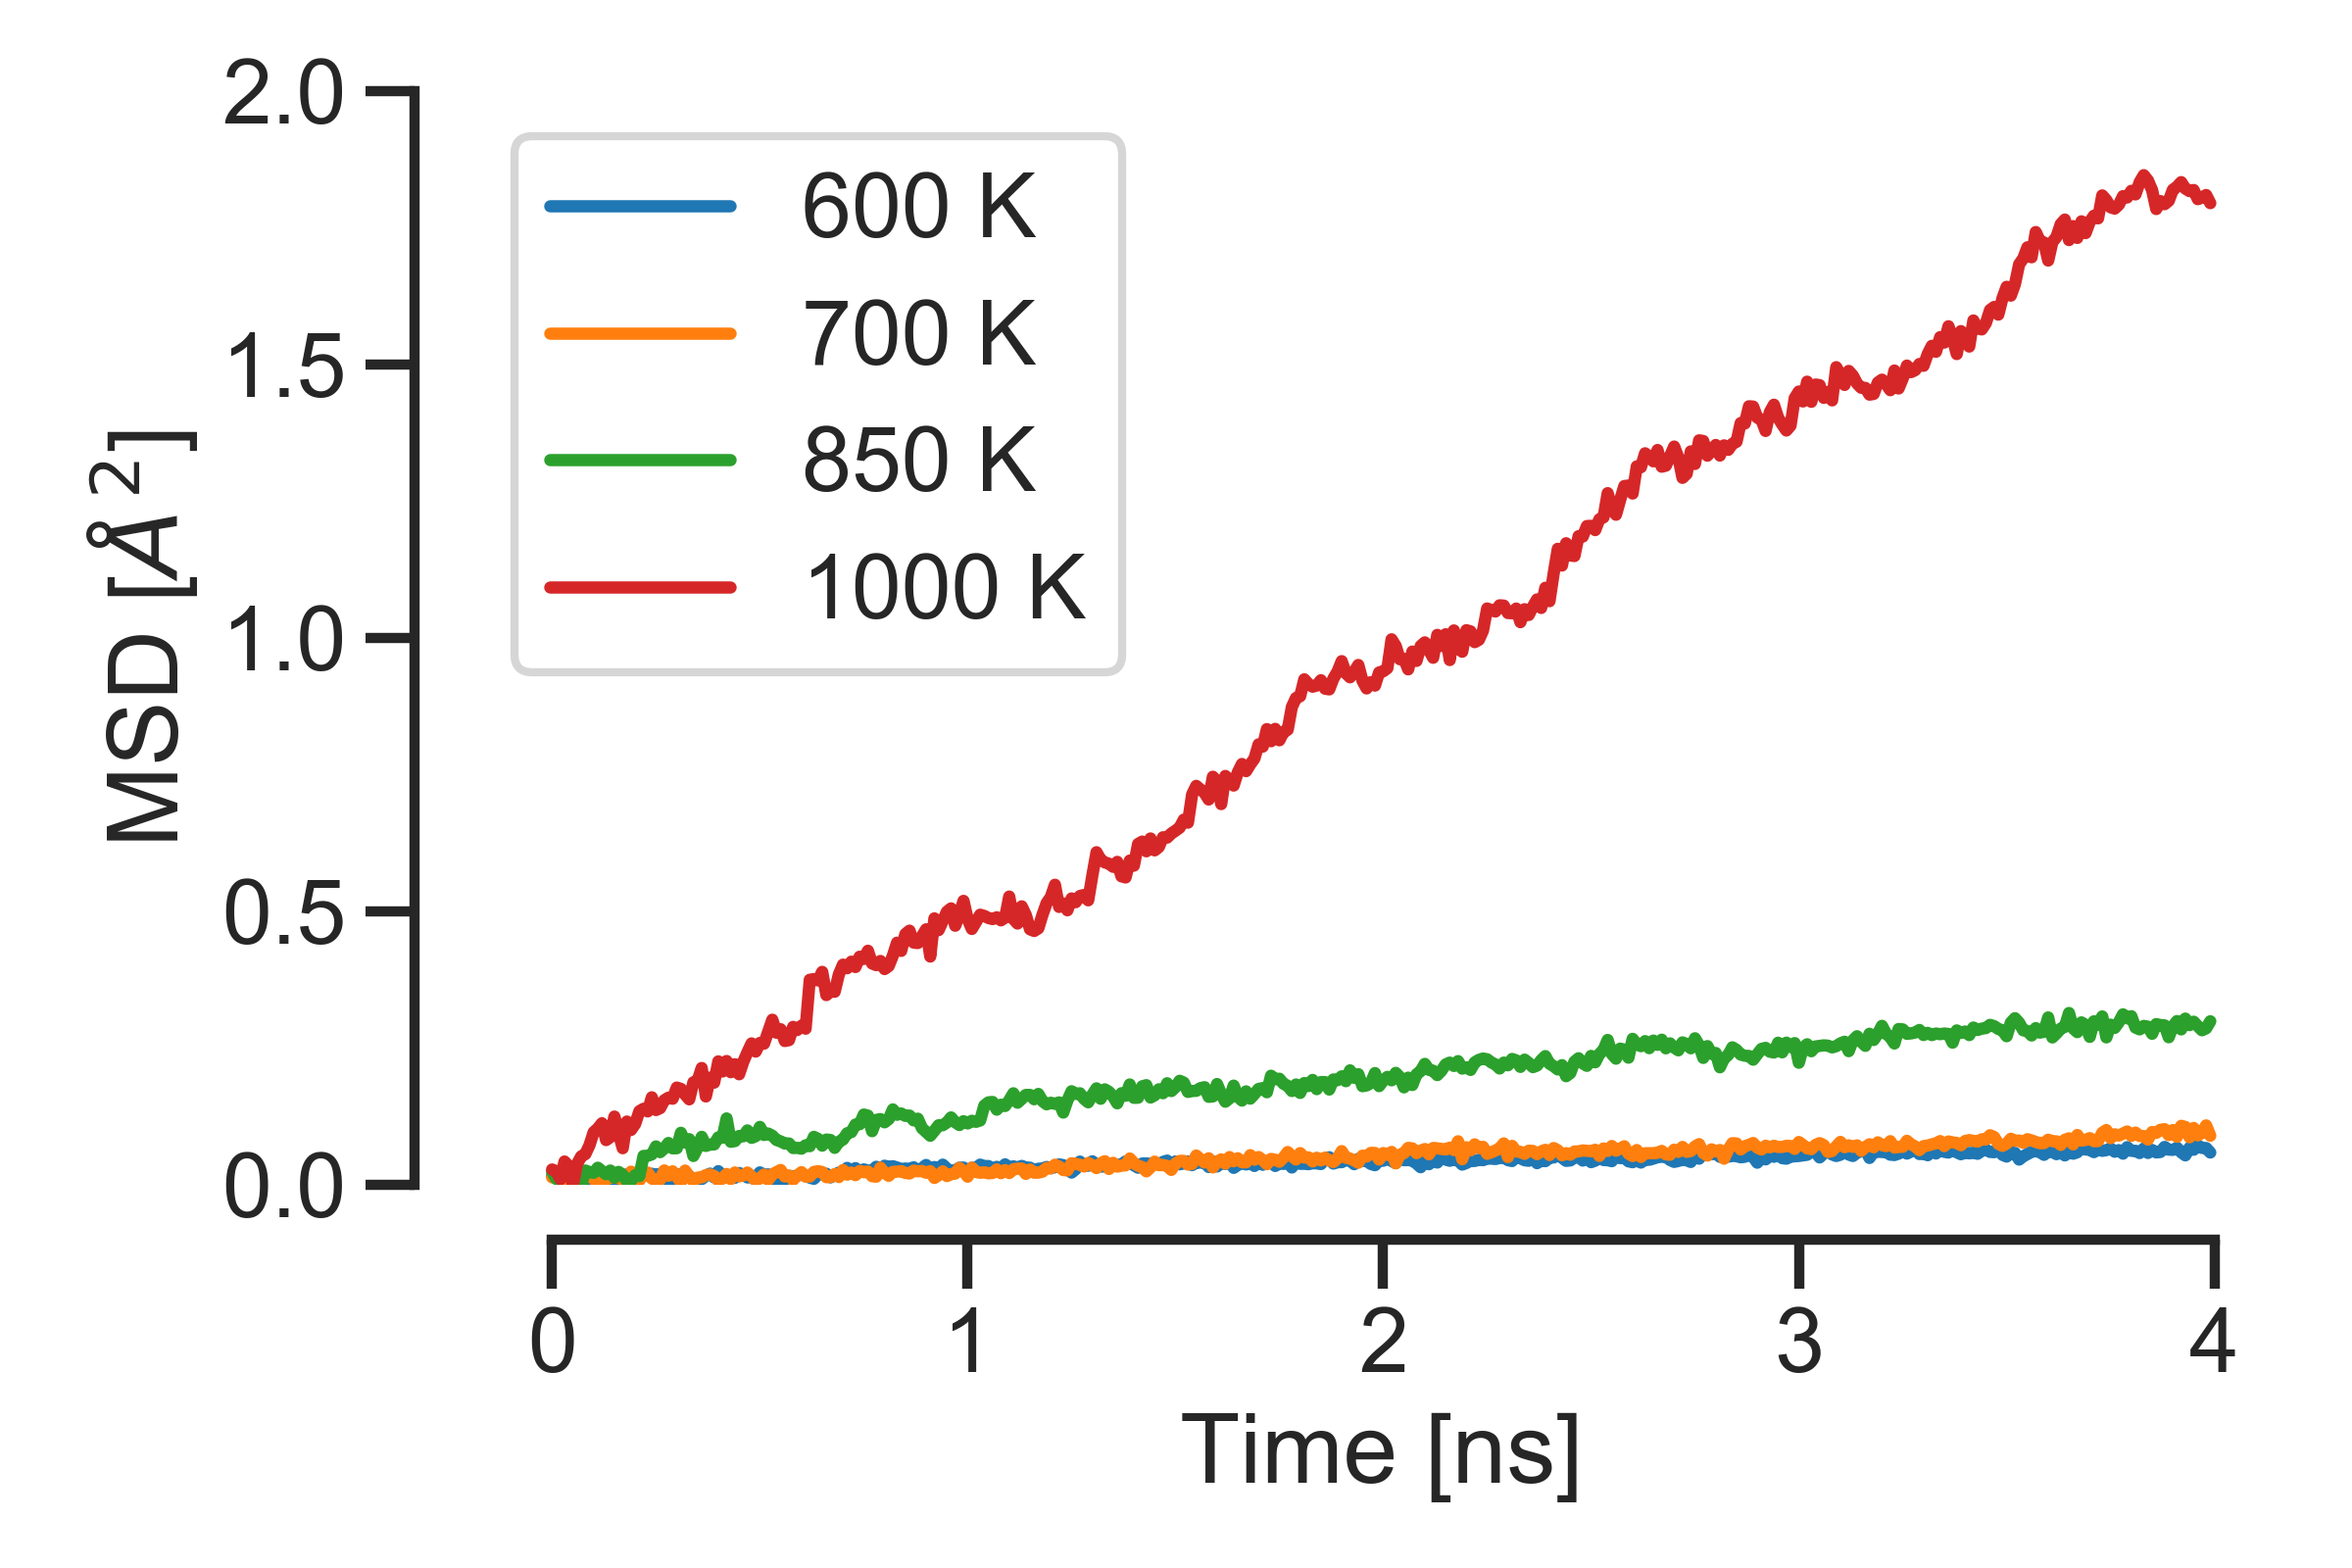
\includegraphics[width=0.8\linewidth]{figures/static/MSD_all}
\caption{MSD plots of lithium ion diffusion in 10\% delithiated \ce{Li4Mn2O5} at a range of temperatures.}
\label{fig:msdall}
\end{figure}

\begin{figure}[p]
\centering
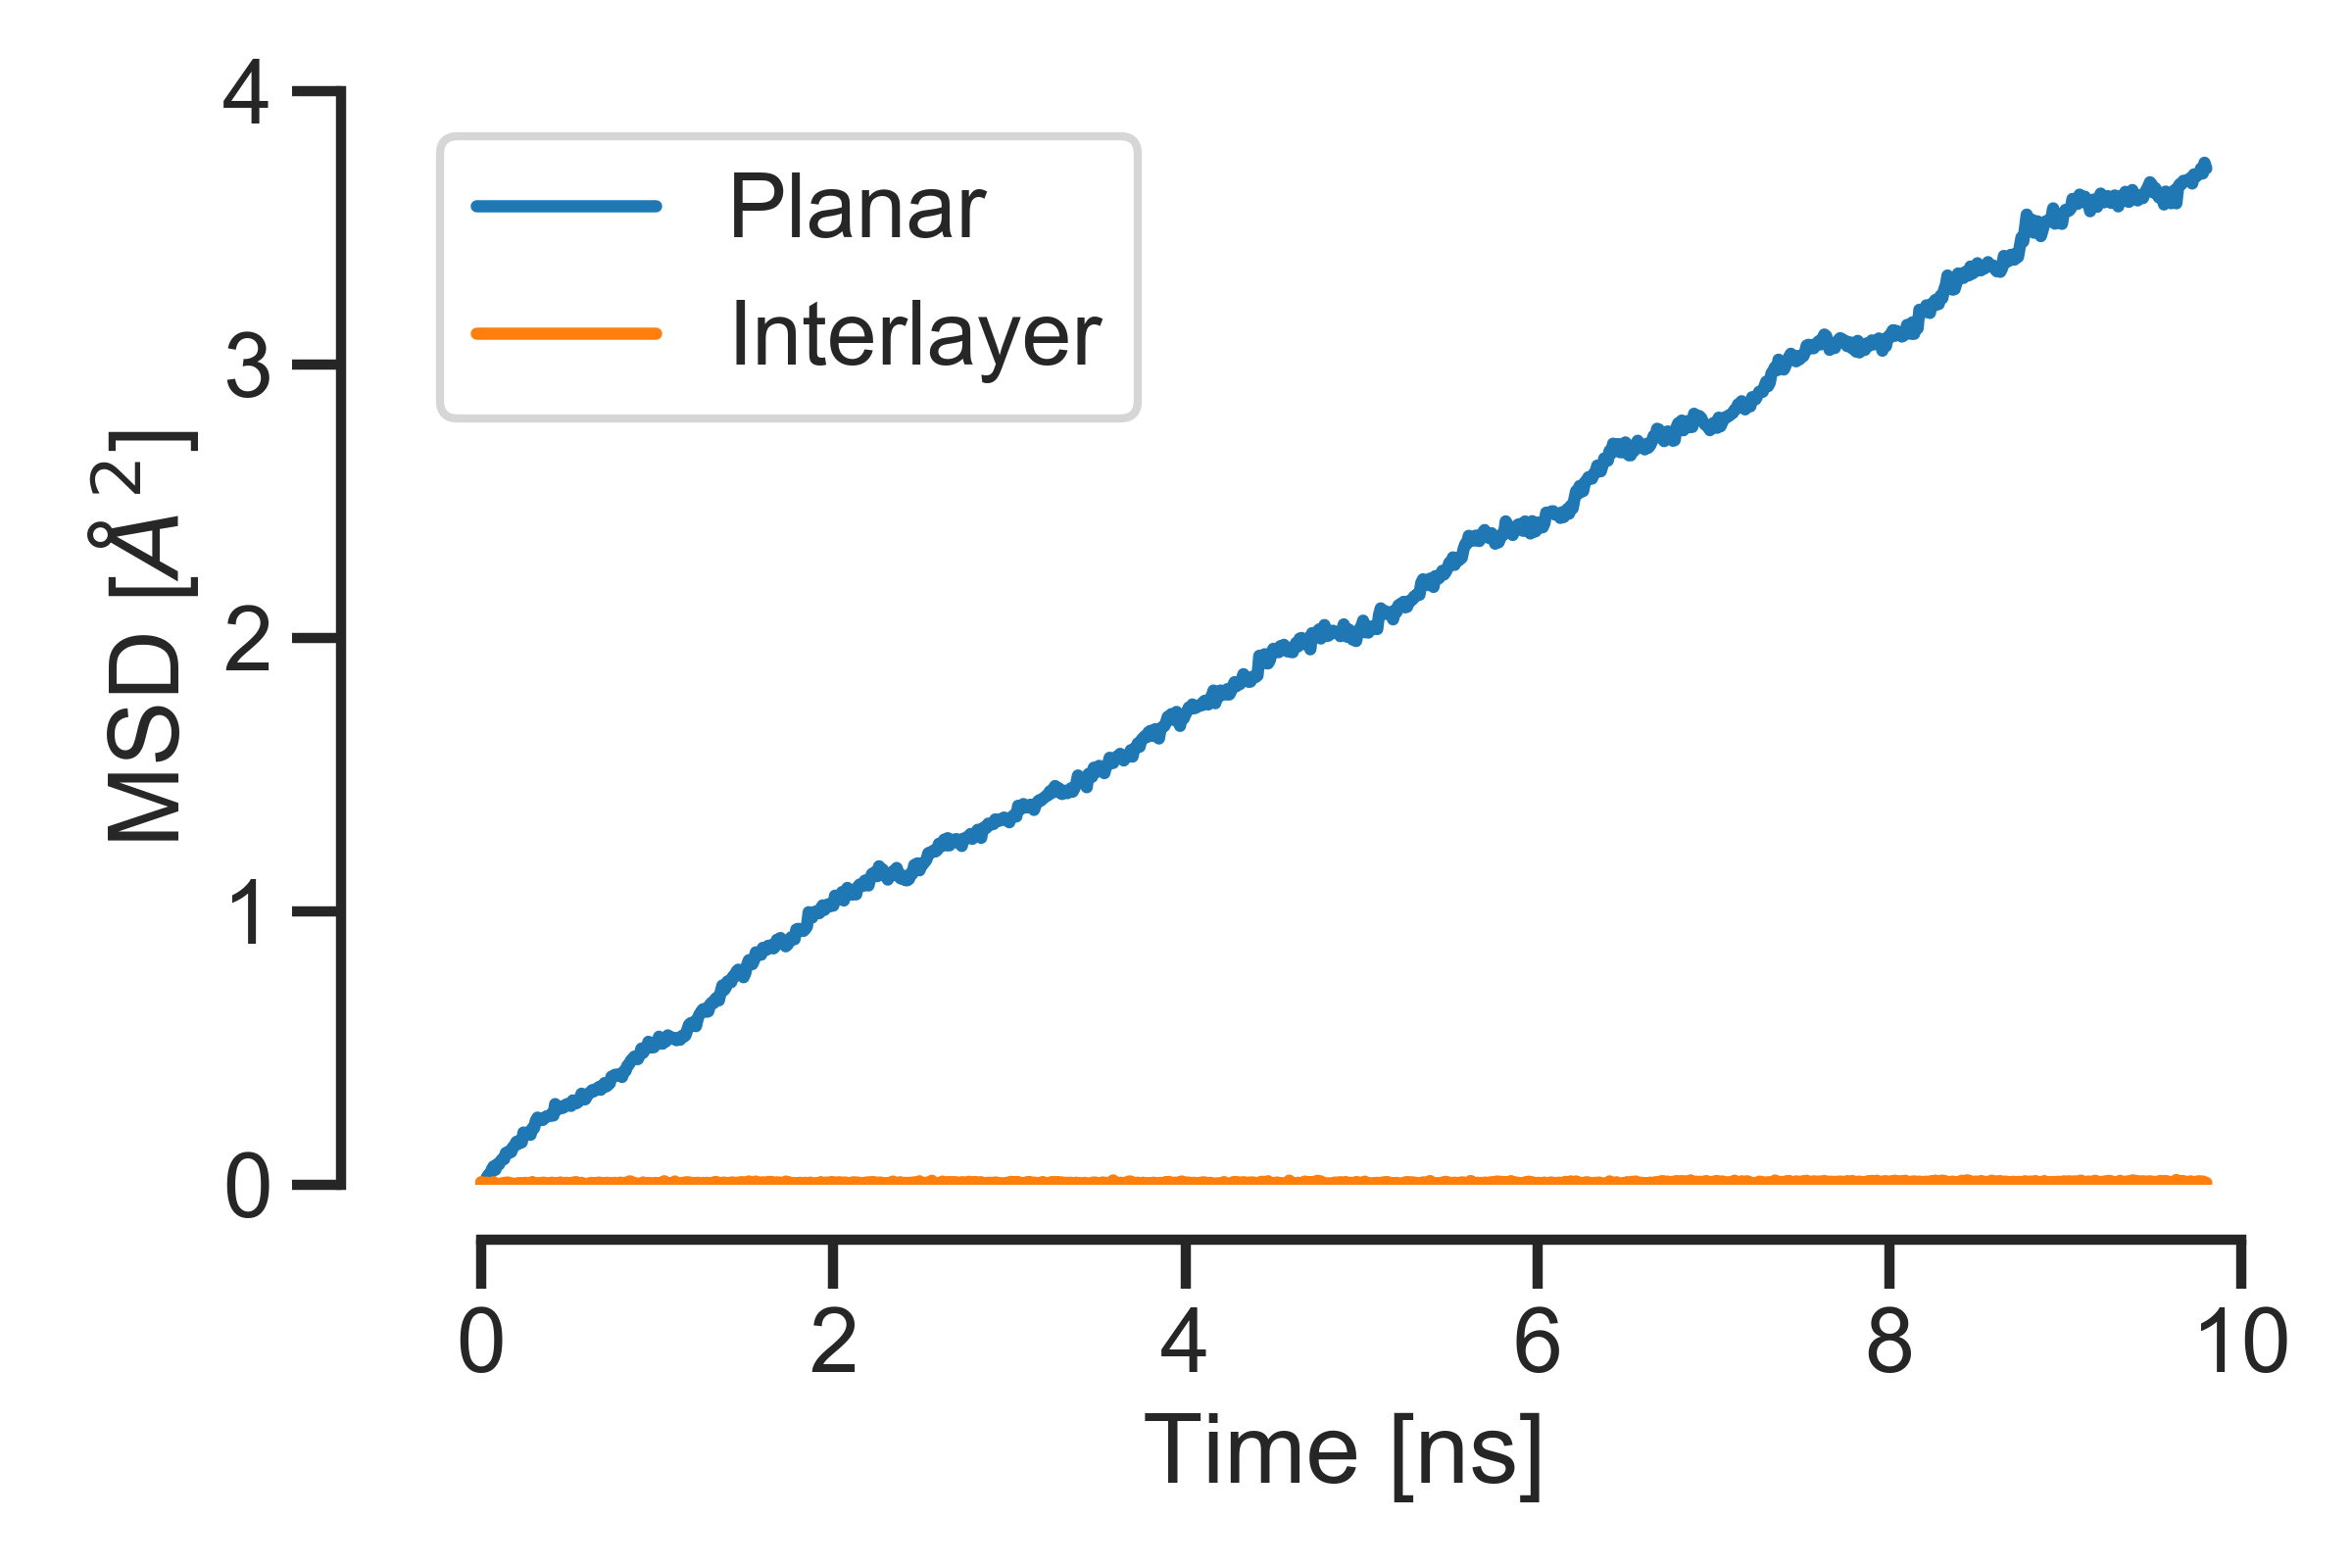
\includegraphics[width=0.8\linewidth]{figures/static/MSD_1000}
\caption{MSD plots of lithium ion diffusion at \SI{1000}{\kelvin} in 10\% delithiated \ce{Li4Mn2O5} for both planar and interlayer motion.}
\label{fig:msd1000}
\end{figure}

\begin{figure}[p]
\centering
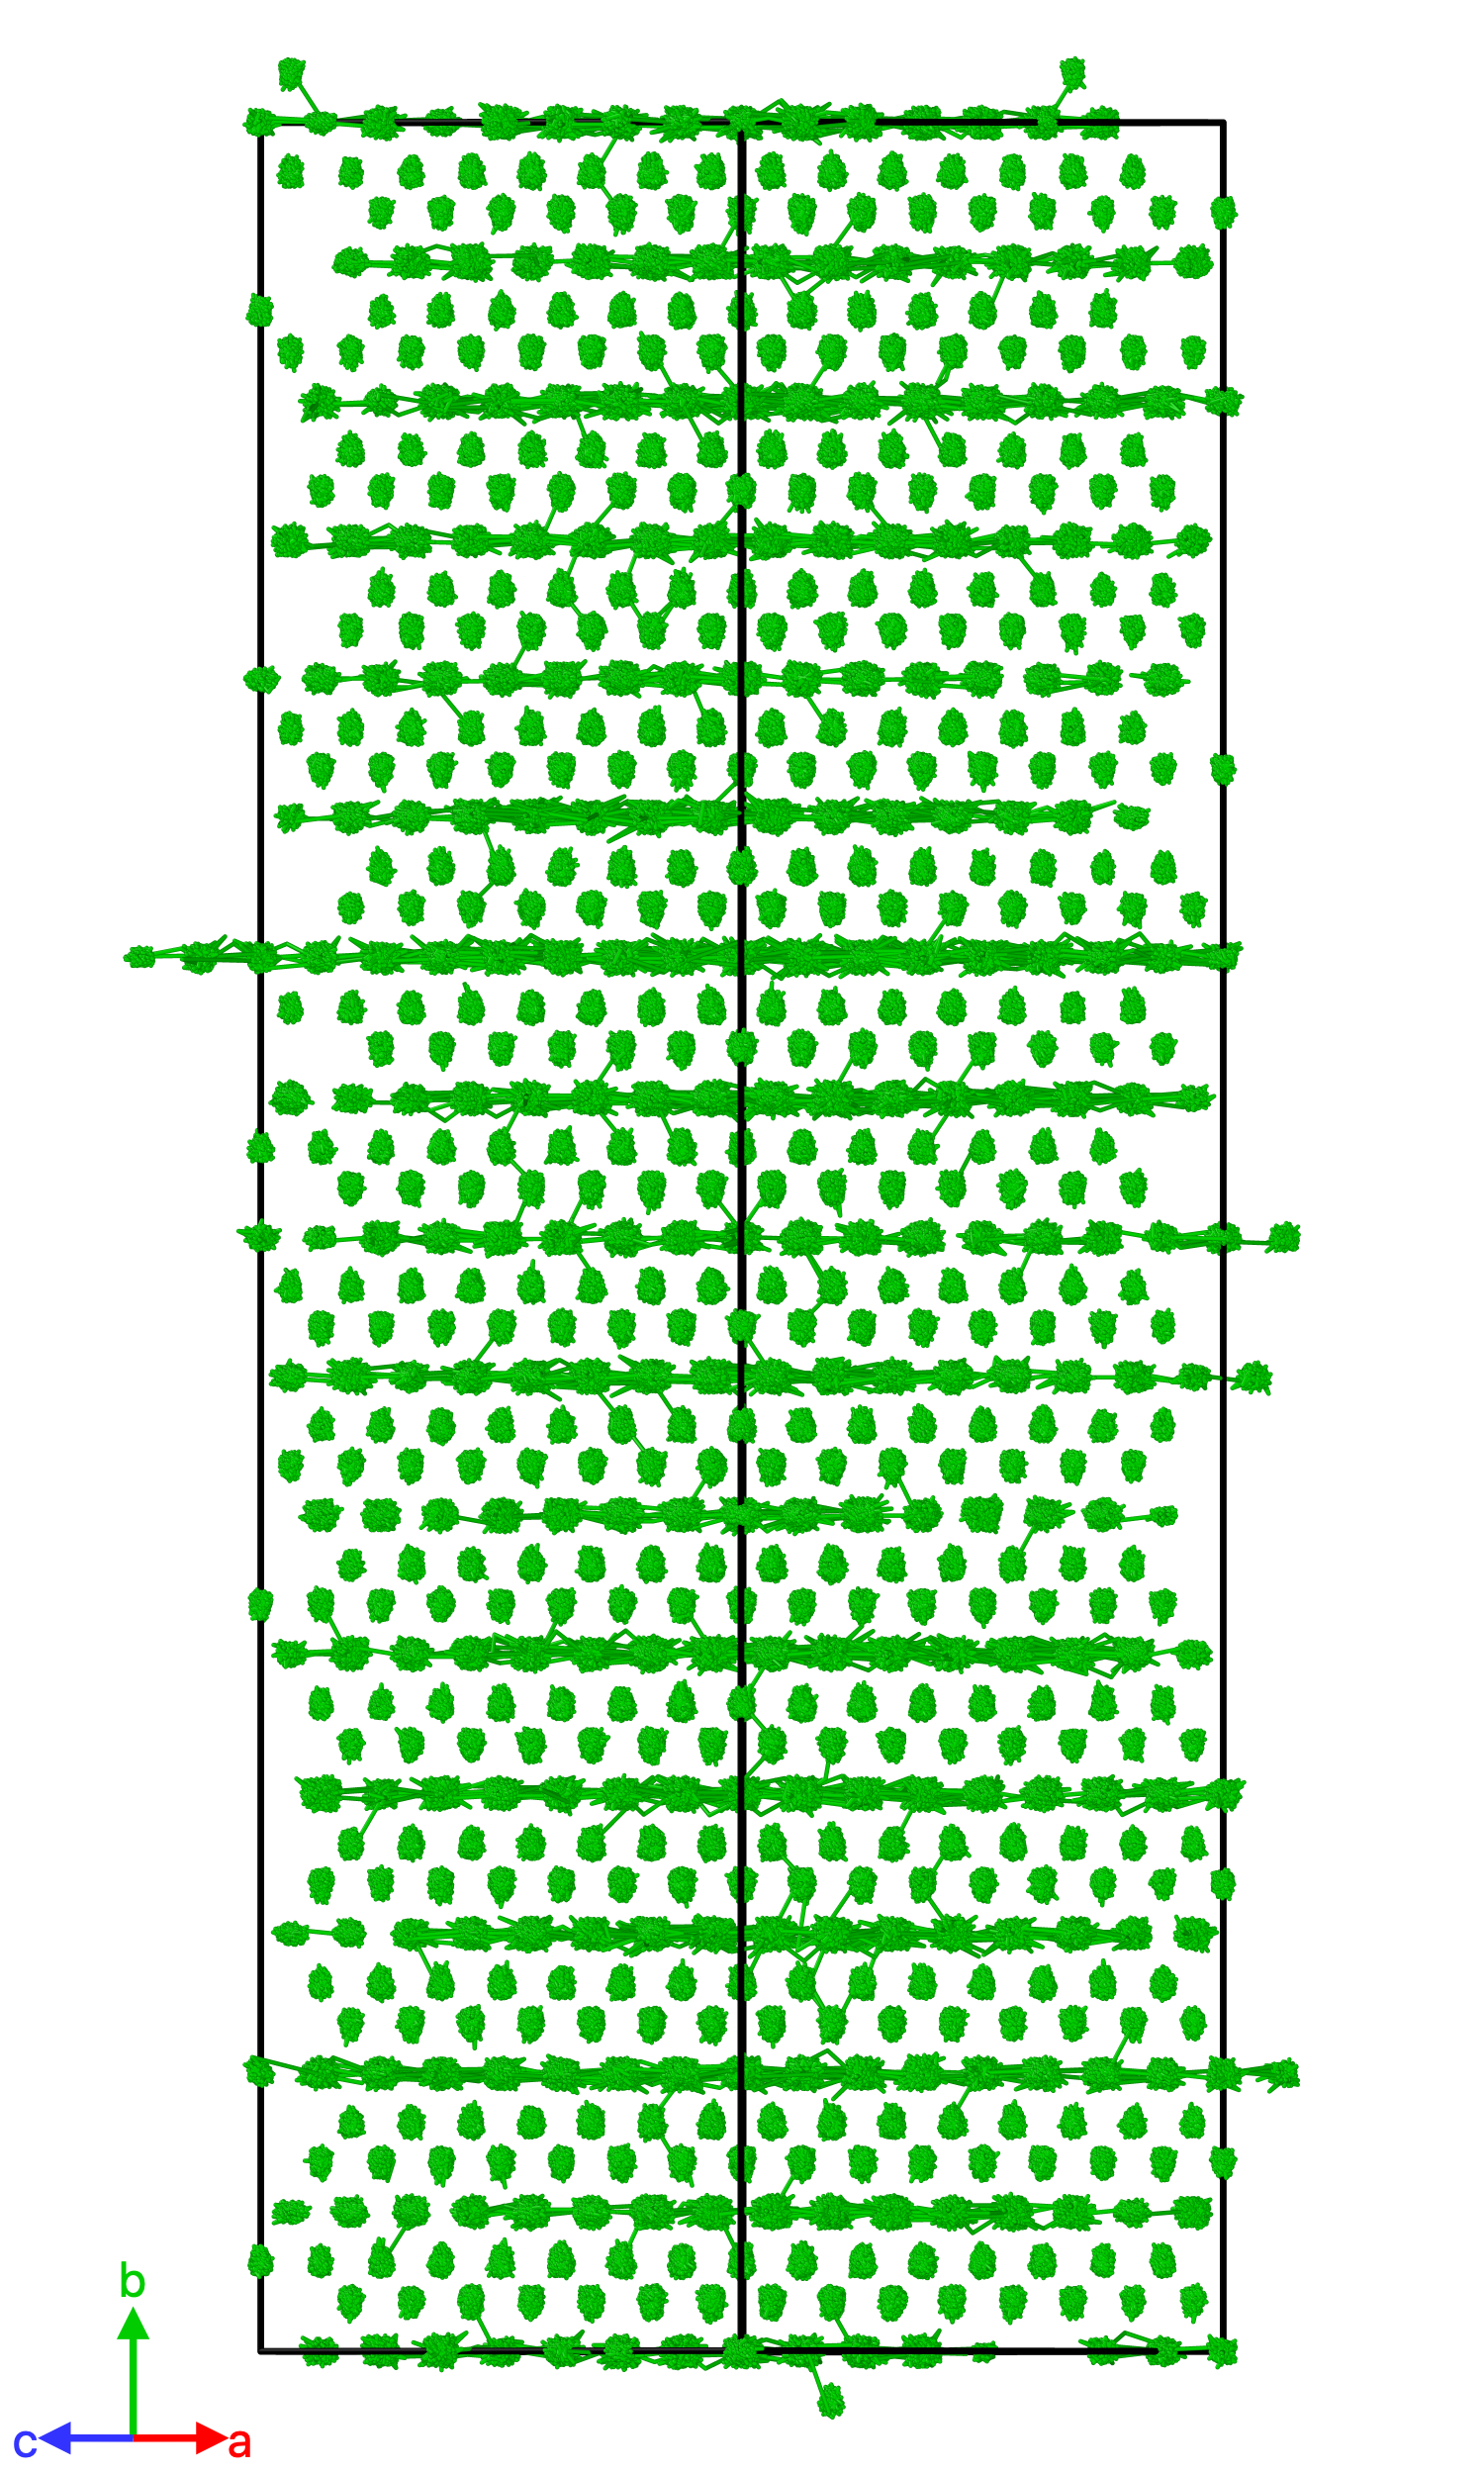
\includegraphics[height=0.85\textheight]{figures/static/trace_portrait}
\caption{Trajectories of lithium ions over a 5 ns period in an MD simulation of ordered \ce{Li4Mn2O5} at 1000K. The vast majority of lithium migration events observed occur in the ac plane.}
\label{fig:trajectory}
\end{figure}


\newpage
\section{Chapter summary and conclusions}
This chapter has used well-established atomistic modelling techniques to provide atomic scale insights into the energetics of defect formation and lithium ion migration in \ce{Li4Mn2O5}.
The disordered nature of \ce{Li4Mn2O5} leads to the formation of a range of local environments, which are not readily replicated due to lack of prior knowledge of the formation energies of these environments.
\ce{Li4Mn2O5} is a promising cathode candidate, but its highly disordered structure poses some significant barriers to the use of potentials based simulation techniques in its characterisation.
The findings of this work are summarised as follows:

\begin{itemize}
	\item Structural modelling can be performed using either the mean-field approximation or ordered approximations of \ce{Li4Mn2O5}, but purely random structure generation does not reproduce the rock-salt structure seen in experimental work.
	\item The ordered approximations of \ce{Li4Mn2O5} exhibit high formation energies for both Schottky and Frenkel type defects, suggesting that neither would be present at a high concentration in the bulk material at typical operating temperatures.
	
	\item Neither random structure generation nor the use of ordered approximations of disordered \ce{Li4Mn2O5} can adequately recreate the random isotropic and low-energy percolation networks of lithium pathways characteristic of disordered rock-salt cathode materials.
	\item A need for quasi-random structure generation techniques which account for the energetics of local environments has been identified, if the mobility of lithium in \ce{Li4Mn2O5} is to be studied.
\end{itemize}



\newpage